\section{Stratified case}
In this section, we no longer assume that the stratification
is neutral. The effect of humidity is neglected.
We first discuss the continuous and semi-discrete in space
equations, then give the
profile of viscosities depending on the turbulent kinetic energy
(TKE), and extend the previous discussion on the wall Law to
Monin-Obukhov Similarity Theory (MOST).

\subsection{Continuous model and Finite Volumes discretization}
\subsubsection{Continuous model}
The wind speed $u$ and the potential temperature $\theta$ evolve
together with
\begin{equation}
\begin{aligned}
	\label{eq:ND_StratifiedCase_EkmanEq}
  (\partial_t + if) u - \partial_z (\partial_z K_u u) &= if u_G \\
  \partial_t \theta -\partial_z (\partial_z K_{\theta} \theta) &= 0.
\end{aligned}
\end{equation}
The viscosities $K_u, K_\theta$ will be detailed in section \ref{sec:ND_StratifiedCase_turbulentVisc}.
The boundary condition on the fluxes $K_u u$ and $K_\theta \theta$
in the surface layer is
\begin{equation}
\begin{aligned}
	\left.K_u \partial_z u \right|_{z\leq \delta_{\rm sl}}
	&= u_\star^2
	\frac{u(\delta_{\rm sl}, t)}{||u(\delta_{\rm sl}, t)||} \\
	\left.K_\theta \partial_z \theta
	\right|_{z\leq \delta_{\rm sl}}
	&= \theta_\star u_\star = C_H ||u(\delta_{\rm sl})||
	\left(\theta(\delta_{\rm sl}) - \theta_{s}\right)
\end{aligned}
\end{equation}
and MOST profiles are
%{\color{red} A décider/ comprendre}
\begin{equation}
\label{eq:ND_StratifiedCase_MOST}
\begin{aligned}
    ||u(z)|| = \frac{u_\star}{\kappa}
    \left(
	\log(\frac{z}{z_{0M}})
    - \psi_u(\frac{z}{L_{MO}})
	+ \psi_u(\frac{z_{0M}}{L_{MO}})
    \right)
    \\
    \theta(z) - \theta_s = 
    \frac{\theta_\star}{\kappa}
    \left(
	\log(\frac{z}{z_{0H}})
    - \psi_\theta(\frac{z}{L_{MO}})
	+ \psi_\theta(\frac{z_{0H}}{{L_{MO}}})
    \right)
\end{aligned}
\end{equation}
where $L_{MO} = \frac{\theta(\delta_{\rm sl})
u_\star^2}{\theta_\star \kappa g }$. We will use
$C_H|u(\delta_{sl})| = \frac{u_\star \kappa}{\log(\frac{z}{z_{0H}})
    - \psi_\theta(\frac{z}{L_{MO}})
    + \psi_\theta(\frac{z_{0H}}{{L_{MO}}})}$
\subsubsection{Finite Volumes discretization}
The discretization of $u$ is exactly the same as in the
neutral case (\eqref{eq:ND_NeutralCase_semiDiscreteEkmanEq} and \eqref{eq:ND_NeutralCase_prognosticEqFV}) and the discretization of 
the potential temperature is very similar:
the average potential temperature $\overline{\theta}_{m+1/2}$
evolves with
\begin{equation}
\label{eq:ND_StratifiedCase_semiDiscreteEkmanEqPT}
    \partial_t \overline{\theta}_{m+1/2}
    - \frac{K_{\theta, m+1} {(\partial_z \theta)}_{m+1} - K_{\theta, m} {(\partial_z \theta)}_m}{h_{m+1/2}}
    = 0
\end{equation}
And the derivative of temperature at $z_{m-1}, z_m, z_{m+1}$ solves
\begin{equation}
\begin{aligned}
\label{eq:ND_StratifiedCase_prognosticPT_FV}
\partial_t \left( \frac{h_{m-1/2}}{6h_m} {(\partial_z \theta)}_{m-1} 
+ \frac{2}{3} {(\partial_z \theta)}_m  
+ \frac{h_{m+1/2}}{6h_m} {(\partial_z \theta)}_{m+1} \right)& \\
-
    \left(
	\frac{K_{\theta, m+1}}{h_m h_{m+1/2}}{(\partial_z \theta)}_{m+1} - \frac{2 K_{\theta, m}}{h_{m-1/2} h _{m+1/2}}{(\partial_z \theta)}_m + \frac{K_{\theta, m-1}}{h_m h_{m-1/2}}{(\partial_z \theta)}_{m-1}
    \right)
&= 0
\end{aligned}
\end{equation}
\subsection{Turbulent viscosities}
\label{sec:ND_StratifiedCase_turbulentVisc}
The Turbulent Kinetic Energy (TKE) evolves with the equation
\begin{equation}
\label{eq:ND_StratifiedCase_TKE}
    \begin{aligned}
    \partial_t e =
    \underbrace{\partial_z \left(K_e
    \partial_z e\right)}_{\text{diffusion}}
    + \underbrace{K_u ||\partial_z u||^2}_{\text{shear}} 
    - \underbrace{K_{\theta} N^2 }_{\text{buoyancy}}
    - \underbrace{c_{\epsilon}
    \frac{e^{3/2}}{l_{\epsilon}(z)}}_{\text{dissipation}}.
    \end{aligned}
\end{equation}
The turbulent viscosities $K_u, K_{\theta}$ and $K_e$ are computed
with $(K_u, K_\theta, K_e) = (C_m , C_s \phi_z, C_e)l_m \sqrt{e}$.
$l_m, l_\epsilon$ are obtained with the fourth method described in \cite{lemarie2021gmd} (section 4.2.2) named $l^\star_{\rm D80}$.

In the Neutral case, no buoyancy term intervene in the computation
of the TKE.

Let us assume that in each cell, $e$ is not varying too much and
$l_\epsilon$ is constant. We use Patankar's trick
\footnote{
	multiplying buoyancy by $\frac{\overline{e}^{n+1}}{\overline{e}^n}$ when buoyancy is greater than shear
to ensure positivity preservation of $\overline{e}$ {\color{red}[ref ?]
}} even if it does not guarantee positivity of TKE when
dealing with Finite Volumes.
Shear and buoyancy are also assumed to be constant in each cell
({\color{red} rough approximations}):
\begin{equation}
\label{eq:ND_StratifiedCase_SemiDiscreteTKE}
    \left(
    \frac{c_\epsilon \sqrt{\overline{e}^n}}{l_\epsilon}
	+ {\rm Ptk} \frac{K_{\theta} N^2}{\overline{e}^n}
    + \partial_t
    \right) \overline{e}
    =\frac{K_{e,m+1} (\partial_z e)_{m+1} -
    K_{e,m} (\partial_z e)_{m}}{h_{m+1/2}}
    + K_u ||\partial_z u||^2
    - (1 - {\rm Ptk}) K_\theta N^2
\end{equation}
Where ${\rm Ptk}=1$ if $K_u ||\partial_z u||^2 \leq K_\theta N^2$, 
otherwise ${\rm Ptk}=0$.
Similarly to $\theta$ and $u$, the prognostic equation
to find the spatial derivative of the TKE at 
the borders of the cells is
\begin{equation}
\label{eq:ND_StratifiedCase_prognosticTKE_FV}
\begin{aligned}
&\partial_t
\left(
    h_{m-1/2}\frac{(\partial_z e)_{m-1}}{12}+
    h_m\frac{10(\partial_z e)_{m}}{12}+
    h_{m+1/2}\frac{(\partial_z e)_{m+1}}{12}
\right)
\\&-
    \left(\frac{K_{e,m+1} (\partial_z e)_{m+1} -
        K_{e,m} (\partial_z e)_{m}}{h_{m+1/2}}
-
    \frac{K_{e,m} (\partial_z e)_{m} -
        K_{e,m-1} (\partial_z e)_{m-1}}{h_{m-1/2}}
        \right)
\\
&- \left(K_{u} ||\partial_z u||^2
-  K_\theta N^2 
\left({\rm Ptk}
\left(\frac{\overline{e}}{\overline{e}^n} - 1\right)
+ 1\right)
- \frac{c_\epsilon \sqrt{\overline{e}}}{l_\epsilon} \overline{e}
\right)_{dm} = 0
\end{aligned}
\end{equation}
where the index $X_{dm}$ is a shortcut for $X_{m+1/2} - X_{m-1/2}$.

\paragraph{Boundary conditions}
In the surface layer, $e$ is constant
and $e(z\leq \delta_{\rm sl}) = e_{\rm sl} = \frac{{u_\star}^2}{\sqrt{c_m c_\epsilon}}$.
A homogeneous Neumann boundary condition is used at the top.
Let $k$ be the space index such that
$z_k < \delta_{\rm sl} < z_{k+1}$. The space derivative of e for
$z \leq z_k$ is set to 0 and its average is set to $e_{\rm sl}$.
Let $\widetilde{e}$ be the TKE average on
$[\delta_{\rm sl}, z_{k+1}]$.
We use as a boundary condition $\widetilde{e} - 5 \widetilde{h}
\frac{ (\partial_z e)_k}{12} -
\widetilde{h}\frac{ (\partial_z e)_{k+1}}{12}= e(z<\delta_{sl})$
and $(\partial_z e)_k = 0$.

\subsection{FV free}

We now have all the ingredients to construct a boundary condition
that is coherent with the MOST profiles with a free
$\delta_{sl}$. Let $k$ such that $z_k < \delta_{\rm sl} < z_{k+1}$.
We assume that
\eqref{eq:ND_StratifiedCase_MOST} apply for $z<\delta_{sl}$,
which leads us to separate the 
cell $[\delta_{\rm sl}, z_{k+1}]$
into two parts: the surface layer $[z_k,\delta_{\rm sl}]$ and the
"subcell" $[\delta_{\rm sl}, z_{k+1}]$ of size $\widetilde{h}$, of
average $\widetilde{u}, \widetilde{\theta}$
and of subgrid reconstructions
\begin{equation}
\begin{aligned}
{\cal S}_{k+1/2}(\xi) = \widetilde{u} +
	\frac{\phi_{k+1} + \phi_{k}}{2} \xi
+ \frac{\phi_{k+1} - \phi_{k}}{2\widetilde{h}}
	\left(\xi^2 - \frac{\widetilde{h}^2}{12}\right) \\
{\cal T}_{k+1/2}(\xi) = \widetilde{\theta}_{1/2} +
	\frac{{(\partial_z \theta)}_{k+1} + 
		{(\partial_z \theta)}_{k}}{2} \xi
+ \frac{{(\partial_z \theta)}_{k+1} - {(\partial_z \theta)}_{k}}
	{2\widetilde{h}}
	\left(\xi^2 - \frac{\widetilde{h}^2}{12}\right)
\end{aligned}
\end{equation}
Here, $\xi = z - (z_{k+1} - \frac{\widetilde{h}}{2})$.
The relation between
$\overline{u}_{k+1/2}, \overline{\theta}_{k+1/2}$ and
$\widetilde{u},\widetilde{\theta}$ is, similarly to the neutral case:
\begin{equation} \label{eq:ND_StratifiedCase_tmprelation_tilde_bar}
\begin{aligned}
\frac{\widetilde{h}}{h_{k+1/2}} \widetilde{u} =
	\overline{u}_{k+1/2} - u(\delta_{sl}) \tau_{sl, u}\\
\frac{\widetilde{h}}{h_{k+1/2}} (\widetilde{\theta} - \theta_s) =
	(\overline{\theta}_{k+1/2}-\theta_s) -
	(\theta(\delta_{sl})-\theta_s)\tau_{sl, \theta}
\end{aligned}
\end{equation}
with for $x = u, \theta$:
\begin{equation}
\tau_{sl, x}^0 = \frac{\frac{1}{{h_{1/2}}}\int_{z_k}^{\delta_{sl}} \log(1+\frac{z}{z_{0x}})- \psi_x(\frac{z}{L_{MO}})
	dz}{\log(1+\frac{\delta_{sl}}{z_{0x}})- \psi_x(\frac{\delta_{sl}}{L_{MO}})
    }
    =
 \frac{\frac{1}{{h_{1/2}}}
    \left[
	    (z+z_{0x})\log(1+\frac{z}{z_{0x}})-z
    +
    z \Psi_m(\frac{z}{L_{MO}}) \right]_{z_k}^{\delta_{sl}}
    }{\log(1+\frac{\delta_{sl}}{z_{0x}})- \psi_x(\frac{\delta_{sl}}{L_{MO}})
    }
\end{equation}
and
    $\alpha_{sl, x} = \frac{\widetilde{h}_{1/2}}{h_{1/2}} +
    \tau_{sl, x}$
non-dimensional numbers.
Let us inject $u(\delta_{sl}) =
{\cal S}(-\frac{\widetilde{h}}{2})$ and
$\theta(\delta_{sl}) = {\cal T}(-\frac{\widetilde{h}}{2})$:
\begin{equation}
\begin{aligned}
\label{eq:ND_StratifiedCase_relation_tilde_bar}
\alpha_{sl, u}\widetilde{u} = \overline{u}_{k+1/2} +
	\tau_{sl, u}
\widetilde{h}
	(\phi_k/3 + \phi_{k+1}/6) \\
\alpha_{sl, \theta}
\widetilde{\theta}
= \overline{\theta}_{k+1/2} + \tau_{sl, \theta}
	\widetilde{h}(\frac{{(\partial_z \theta)}_k}{3} + \frac{{(\partial_z \theta)}_{k+1}}{6})
 - (1 - \alpha_{sl, \theta})\theta_s
\end{aligned}
\end{equation}

The scheme can then use as boundary conditions at the surface layer:
\begin{equation}
\label{eq:ND_StratifiedCase_boundaryConditionFVfree}
\begin{aligned}
	K_{u,k} \phi_k = {u_\star}^2
  \frac{\overline{u}_{k+1/2} - \frac{\widetilde{h}^2}{h_{k+1/2}}
	(\frac{\phi_k}{3} + \frac{\phi_{k+1}}{6})}
	{\alpha_{sl, u}||u^n(\delta_{sl})||} \\
  \frac{\alpha_{sl, \theta} }
  {C_H |u(\delta_{sl})|}
	K_{\theta, k} (\partial_z \theta)_k = 
  \overline{\theta}_{k+1/2} - \frac{\widetilde{h}^2}{h_{k+1/2}}
	(\frac{{(\partial_z \theta)}_k}{3} +
	\frac{{(\partial_z \theta)}_{k+1}}{6}) 
  - \theta_s\\
\end{aligned}
\end{equation}
Finally, the scheme at the first grid level above
the surface layer is for $u$:
\begin{equation}
\label{eq:ND_StratifiedCase_prognosticu_FVfree}
    \begin{aligned}
(\partial_t + if)
	    \left(\frac{\widetilde{h}}{6h_{k+1}} 
    \phi_k
    +
    \left(
	    \frac{\widetilde{h}}{3h_{k+1}} 
	    + \frac{h_{k+3/2}}{3h_{k+1}}
    \right)
	    \phi_{k+1}
	    + \frac{h_{k+3/2}}{6h_{k+1}} \phi_{k+2}\right)
    = \\
	    \frac{K_{u, k+2} \phi_{k+2} - K_{u, k+1} \phi_{k+1}}
	    {h_{k+3/2}h_{k+1}} - \frac{K_{u, k+1} \phi_{k+1} -
	    K_{u,k} \phi_k }{\widetilde{h}h_{k+1}}
    \end{aligned}
\end{equation}
\begin{equation}
	\label{eq:ND_StratifiedCase_semiDiscreteEkmanEqFVfree}
	\partial_t \left(\frac{1}{\alpha_{\rm sl, u}}
	\left(\overline{u}_{k+1/2} + \widetilde{h}\tau_{\rm sl, u}
	(\frac{\phi_k}{3} + \frac{\phi_{k+1}}{6})\right)\right)
	= \frac{K_{u, k+1}\phi_{k+1} - K_{u,k} \phi_k}{\widetilde{h}}
\end{equation}
and the same applies for $\theta$:
\begin{equation}
\label{eq:ND_StratifiedCase_prognosticPT_FVfree}
    \begin{aligned}
\partial_t \left(\frac{\widetilde{h}}{6h_{k+1}} 
	    {(\partial_z \theta)}_k
    +
    \left(
	    \frac{\widetilde{h}}{3h_{k+1}} 
	    + \frac{h_{k+3/2}}{3h_{k+1}}
    \right)
	    {(\partial_z \theta)}_{k+1}
	    + \frac{h_{k+3/2}}{6h_{k+1}} {(\partial_z \theta)}_{k+2}\right)
    = \\
	    \frac{K_{\theta, k+2} {(\partial_z \theta)}_{k+2} -
	    K_{\theta, k+1} {(\partial_z \theta)}_{k+1}}
	    {h_{k+3/2}h_{k+1}} - \frac{K_{\theta, k+1} {(\partial_z \theta)}_{k+1} -
	    K_{\theta, k} {(\partial_z \theta)}_k }{\widetilde{h}h_{k+1}}
    \end{aligned}
\end{equation}
\begin{equation}
	\label{eq:ND_StratifiedCase_semiDiscreteEkmanEqPTFVfree}
	\partial_t \left(\frac{1}{\alpha_{\rm sl, \theta}}
	\left(
	\overline{\theta}_{k+1/2} + \tau_{sl, \theta}
	\widetilde{h}(\frac{{(\partial_z \theta)}_k}{3} +
	\frac{{(\partial_z \theta)}_{k+1}}{6})
	 - (1 - \alpha_{sl, \theta})\theta_s
	\right) \right)
	= \frac{K_{\theta, k+1}{(\partial_z \theta)}_{k+1} -
	K_{\theta,k} {(\partial_z \theta)}_k}{\widetilde{h}}
\end{equation}

\begin{figure}
	\centering
	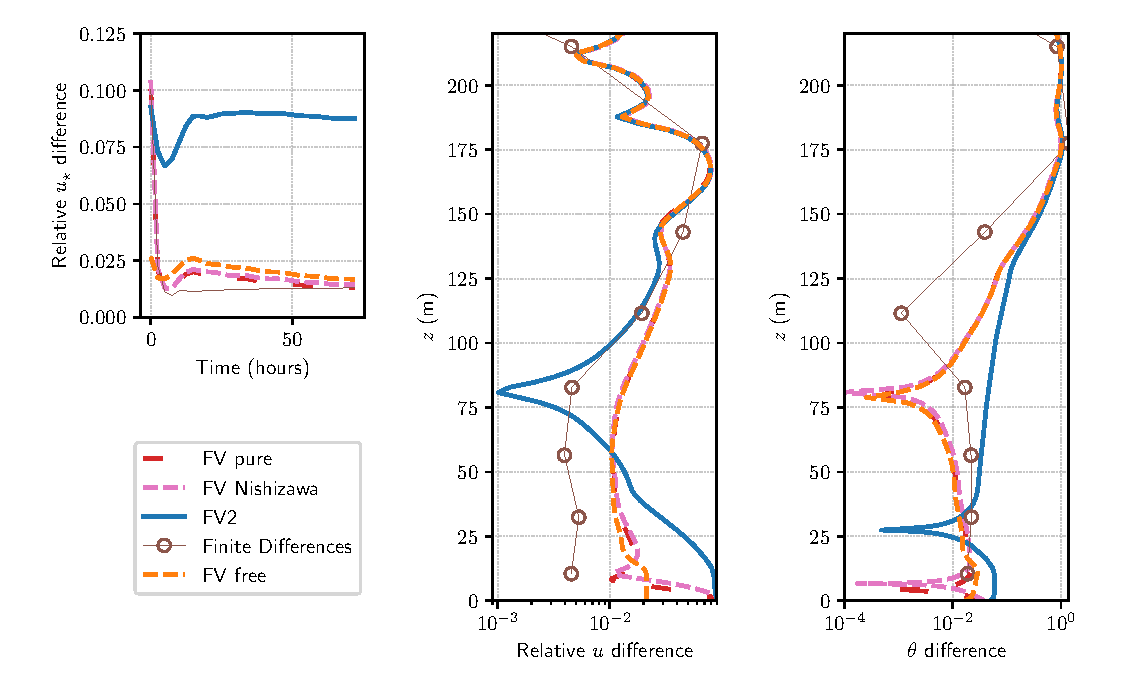
\includegraphics[scale=0.55]{images/consistency_comparisonStratified.pdf}
	\includegraphics[scale=0.55]{images/consistency_comparisonStratified_linearscale.pdf}
	\caption{Stratified (stable) case's numerical experiment. Top: log-scaled, bottom: linear-scaled}
	\label{fig:ND_StratifiedCase_NumericalExpStable}
\end{figure}
\begin{figure}
	\centering
	\includegraphics[scale=0.55]{images/consistency_comparisonUnstable.pdf}
	\caption{Stratified (unstable) case's numerical experiment.}
	\label{fig:ND_StratifiedCase_NumericalExpUnstable}
\end{figure}

\subsection{Matching viscosities at the surface layer}
In order to obtain a regular solution out of the "FV free"
discretization, we derive here the constraints on mixing length
and on TKE inside the surface layer.
Assuming that 
\begin{equation}
	\label{eq:ND_StratifiedCase_viscosities_assumption}
K_m = C_m l_m \sqrt{e} ~~\text{and}~~
K_\theta = C_s l_m \sqrt{e} \phi_z
\end{equation}
 inside the SL, we have
for $z\leq \delta_{\rm sl}$
\begin{enumerate}
\item Constant flux layer hypothesis and Robin boundary condition:
\begin{subequations}
\begin{equation}
	\label{eq:ND_StratifiedCase_K_partial_z_u}
	K_m \partial_z u = u_\star^2 \frac{u(\delta_{sl})}{|u^n(\delta_{sl})|}
\end{equation}
\begin{equation}
	\label{eq:ND_StratifiedCase_partial_z_u}
	\partial_z u = u_\star \frac{\phi_m(z/L_{MO})}{\kappa (z + z_{0M})}\frac{u(\delta_{sl})}{|u^n(\delta_{sl})|}
\end{equation}
\begin{equation}
	\label{eq:ND_StratifiedCase_partial_z_theta}
	\partial_z \theta = \theta_\star \frac{\phi_h(z/L_{MO})}{\kappa (z + z_{0H})}, ~~~ K_\theta \partial_z \theta = u_\star \theta_\star
\end{equation}
\end{subequations}
Leading to 
\begin{equation}
	\label{eq:ND_StratifiedCase_viscosities_SL}
	K_m = \kappa u_\star\frac{z+ z_{0M}}{\phi_m(z/L_{MO})} ~~\text{and}~~
K_\theta = \kappa u_\star\frac{z+ z_{0M}}{\phi_h(z/L_{MO})}
\end{equation}
\eqref{eq:ND_StratifiedCase_viscosities_assumption}
together with \eqref{eq:ND_StratifiedCase_viscosities_SL} put
a constraint on $\phi_z$ in the surface layer:
$\phi_z = \frac{C_m\phi_m(z/L_{MO})}{C_s\phi_h(z/L_{MO})}
		\forall z\leq \delta_{\rm sl}$.
\item Quasi-equilibrium of the TKE equation:
\begin{equation}
	\label{eq:ND_StratifiedCase_TKE_quasi_equilibrium}
	c_\epsilon \frac{e^{3/2}}{l_\epsilon}=K_m ||\partial_z u||^2 - \frac{g}{\theta_{ref}} K_\theta \partial_z \theta
\end{equation}
\end{enumerate}
We assume that $l_\epsilon$ in
\eqref{eq:ND_StratifiedCase_TKE_quasi_equilibrium} is taken at
time index $n$, so that the energy can be integrated in time
with a proper boundary condition before computing the mixing
length. Then, we assume that $l_m = \sqrt{l_{up}l_{down}}$ and
$l_\epsilon = \min(l_{up}, l_{down})$.
We choose to keep the free-turbulence value
$l_{up}^0 = \frac{2\sqrt{e}}
{c_0|\partial_z u| + \sqrt{c_0^2 |\partial_z u| + 2N^2}}$
in the SL, using \eqref{eq:ND_StratifiedCase_partial_z_u}
to compute $|\partial_z u|$ and using
\eqref{eq:ND_StratifiedCase_partial_z_theta}
for $N^2 = \frac{g}{\theta_{ref}}\partial_z \theta$.
After $l_{up}^0$ has beed computed, as in
\cite{lemarie2021gmd} $l_{up}$ is limited by
the distance to the top and by the distance to a strongly
stratified portion of the air column.
Keeping the same computing routine for $l_{up}$ seems
more natural since its value should not be too much
influenced by a surface below.
\par
Simplifying \eqref{eq:ND_StratifiedCase_TKE_quasi_equilibrium}
with previous equations gives:
\begin{equation}
	\label{eq:ND_StratifiedCase_TKE_quasi_equilibrium_simplified}
	e = \min(l_{up}^{2/3}, l_{down}^{2/3})\left(
	\frac{u_\star}{c_\epsilon} 
	\left({u}_\star^2
	\frac{\phi_m(z/L_{MO})}{\kappa (z+z_{0M})}
	- \frac{g}{\theta_{\rm ref}}\theta_\star
	\right)
	\right)^{2/3}
\end{equation}

Now, \eqref{eq:ND_StratifiedCase_viscosities_SL} gives
\begin{equation}
	\label{eq:ND_StratifiedCase_solution_l_down}
	l_{down}(e) = \frac{1}{l_{up} e} \left(
	\frac{\kappa u_\star}{C_m}
	\frac{z + z_{0M}}{\phi_m(z/L_{MO})}
\right)^2
\end{equation}
$l_{down}$ is limited by the distance to the bottom only
in the free-turbulence zone. In the SL, it keeps its value
\eqref{eq:ND_StratifiedCase_solution_l_down}
so that \eqref{eq:ND_StratifiedCase_viscosities_SL} is
verified.
We inject \eqref{eq:ND_StratifiedCase_TKE_quasi_equilibrium_simplified}
into the previous equation and get
\begin{equation}
	\label{eq:ND_StratifiedCase_solution_l_down}
	\begin{cases}
	l_{down}^{5/3} = \frac{1}{l_{up}} \frac{u_\star^{4/3}\left(
	\frac{\kappa}{C_m}
	\frac{z + z_{0M}}{\phi_m(z/L_{MO})}
	\right)^2}{
	\left({u}_\star^2
	\frac{\phi_m(z/L_{MO})}{c_\epsilon\kappa (z+z_{0M})}
	- \frac{g}{\theta_{\rm ref}c_\epsilon}\theta_\star
	\right)^{2/3}} ~~~ {\rm if } ~~l_{down} < l_{up}\\
	l_{down}(e) = \frac{1}{l_{up}^{5/3}} \frac{u_\star^{4/3}\left(
	\frac{\kappa}{C_m}
	\frac{z + z_{0M}}{\phi_m(z/L_{MO})}
	\right)^2}{
	\left({u}_\star^2
	\frac{\phi_m(z/L_{MO})}{c_\epsilon\kappa (z+z_{0M})}
	- \frac{g}{\theta_{\rm ref}c_\epsilon}\theta_\star
	\right)^{2/3}} ~~~ {\rm otherwise}\\
	\end{cases}
\end{equation}

\subsection{On the value of $K_0$}
\label{sec:ND_StratifiedCase_viscosity0_FVpure}
If we strictly follow the content of this document,
$K_0$ should be equal to $K_{mol}$ (except for the "FV free" case).
However, the boundary condition $K_0 \phi_0 = u_\star^2$
does not behave the same way with FD and FV.
(The orientation $\frac{u(\delta)}{||u(\delta)||}$
was omitted for simplicity purpose. We also assume here $f=0$).

\paragraph{Finite Differences}
Injecting the boundary condition in the first grid level gives
$\partial_t u_{1/2} = \frac{K_1}{h}\left(\frac{u_{3/2} - u_{1/2}}{h}
 - u_\star^2
\right)$.
\textbf{The value of $K_0$ does not directly intervene in the equation}.

\paragraph{Finite Volumes}
In the continuity equation at $z=z_1$, it is used that
$\partial_t u(z_1) = \frac{K_1 \phi_1 - u_\star^2}{h}
+ \frac{h \phi_1}{3} + \frac{h u_\star^2}{6 K_0}$
\textbf{The (small) value of $K_0$ directly appears when we assume the
parabolic profile inside the first grid level.}
As a result, $\partial_t u(z_1)$ scales with $\frac{1}{K_0}$.
That is seen
on previous Figures.
To obtain reasonable profiles, $K_0=K(\delta_{\rm sl})$ can be used
but it does not correspond to the original discretisation choice.
The consequence is that $\phi_0$ would not correspond
to $(\partial_z u)(z_0)$ or $(\partial_z u)(z_{\delta_{sl}})$.


\begin{figure}
	\centering
	\includegraphics[scale=0.55]{images/colorplots_FVlowres.pdf}
	\includegraphics[scale=0.55]{images/colorplots_FVhighres.pdf}
	\caption{Stratified (unstable) case's numerical experiment ("FV free").
	Top: low resolution, bottom: high resolution.
	The resolution of the bottom image does not give the space step.
	}
	\label{fig:ND_StratifiedCase_NumericalExpUnstableColorplot}
\end{figure}

\begin{figure}
	\centering
	\includegraphics[scale=0.55]{images/colorplots_FDlowres.pdf}
	\includegraphics[scale=0.55]{images/colorplots_FDhighres.pdf}
	\caption{Stratified (unstable) case's numerical experiment (FD).
	Top: low resolution, bottom: high resolution
	The resolution of the bottom image does not give the space step.
	}
	\label{fig:ND_StratifiedCase_NumericalExpUnstableColorplot}
\end{figure}
